\chapter[Desenvolvimento]{Desenvolvimento}
\label{ch:desenvolvimento}
O \textit{Power Monitor} surgiu da necessidade da conscientização do gasto energético e da melhor compreensão da conta de luz. Baseado nesse conceito,
foram desenvolvido um \textit{software} que permitirá uma fácil comunicação com qualquer equipamento construído que tenha a finalidade de monitorar a energia elétrica e um \textit{hardware} para demonstração
da comunicação entre ambos. O sistema traz uma forma mais fácil e próxima do consumidor final de se quantificar a energia elétrica consumida em um estabelecimento. No lugar do Quilowatt-hora, medida que é usada atualmente,
o \textit{software} propõe mensurar o gasto energético em reais (R\$), trazendo a realidade do consumo mensal para mais próximo de cada brasileiro.

Nesse capítulo será mostrado todo o passo a passo para o desenvolvimento do \textit{software} e \textit{hardware}, juntamente com a comunicação 
entre ambos, por fim será mostrado os resultados obtidos. 


\section[\textit{Visão Geral}]{\textit{Visão Geral}}\label{visal-geral}

Em resumo pode-se ter uma visão geral de como o ambiente - \textit{software} e \textit{hardware} - funciona observando a \autoref{fig:diagrama-vg}.
O sistema \textit{web} é responsável por fazer a comunicação entre o banco de dados e os dispositivos, já os eletrodomesticos são gerenciados
pelo ESP8266 que possui uma comunicação direta via \textit{websocket} com o sistema \textit{web}.

\begin{figure}[h!]
	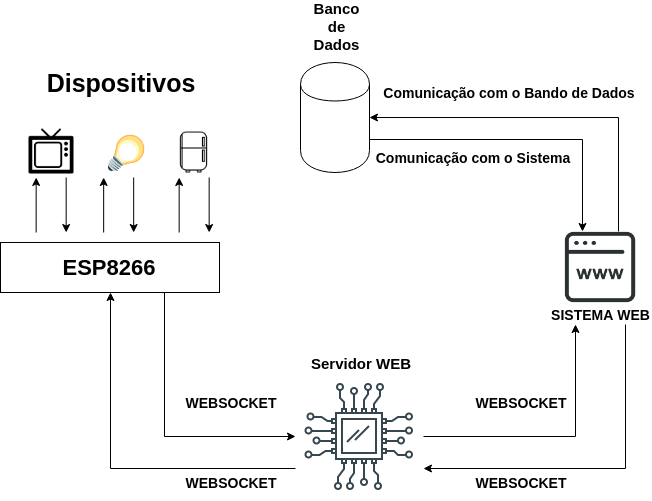
\includegraphics[width=0.7\textwidth, keepaspectratio=true]{diagrama-1}
	\centering
	\caption[Visão geral do ambiente]{Visão geral do ambiente}
	\label{fig:diagrama-vg}
\end{figure}
\FloatBarrier

\section[\textit{Software}]{\textit{Software}}\label{soft-sec}
O controle dos dispositivos de um cômodo, que estão interligados com o \textit{ESP8266} são controlados pelo \textit{software}. Dessa forma
todos os dispositivos que possuem comunicação com o microcontrolador e que estão cadastrados nos sistema podem ser controlados (Ligar/Desligar) e também
é possível ter um acompanhamento dos gastos.

O sistema possui uma interface \textit{web} que pode ser acessada por qualquer dispositivo que tenha acesso a internet e possua um 
\textit{browser}. O \textit{software} possui uma interface de apenas um único usuário, ao acessar o sistema o usuário se depara com um
visual bem agradável e fácil de se usar. Ao entrar no sistema o usuário visualiza a página principal, \autoref{fig:principal-ft}, nela encontram-se
as principais informações que o usuário irá precisar, como também mostrar as oções de cadastrar um novo dispositivo, listar os dispositivos, cadastrar um novo cômodo,
listar um novo cômodo etc.

\begin{figure}[h!]
	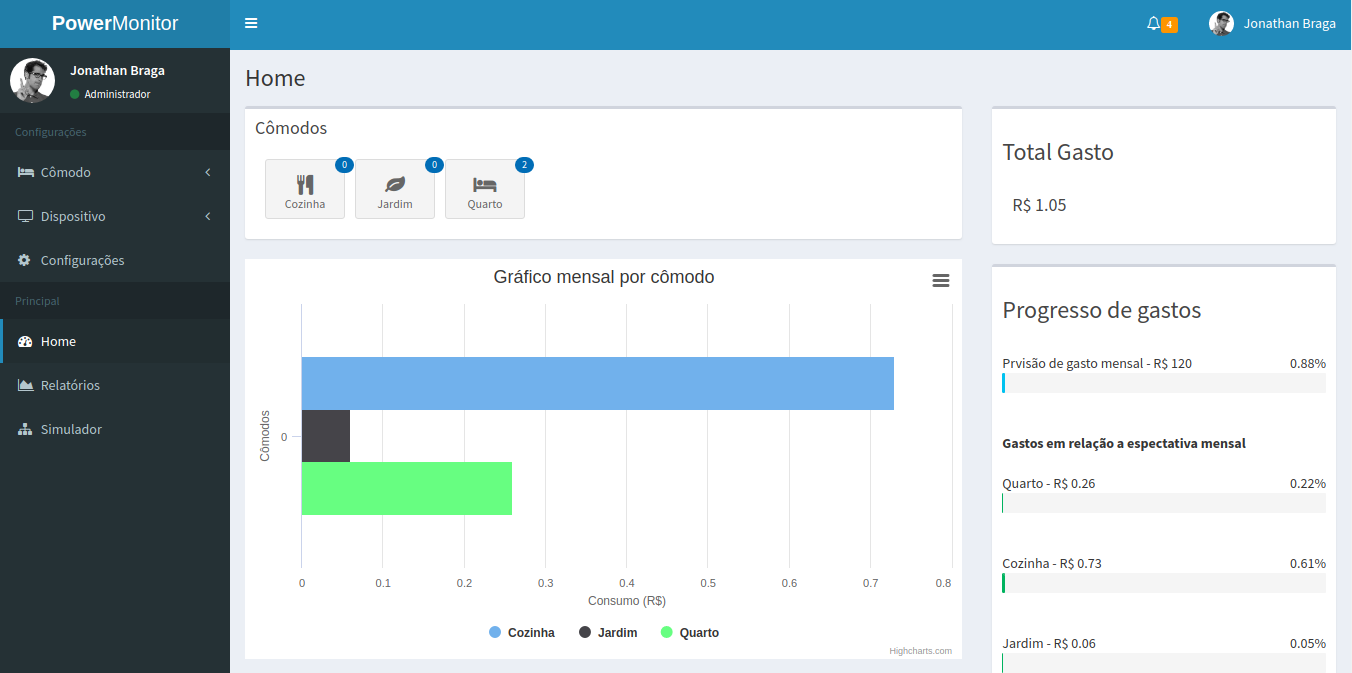
\includegraphics[width=1.0\textwidth, keepaspectratio=true]{principal}
	\centering
	\caption[Tela inicial do sistema]{Tela inicial do sistema}
	\label{fig:principal-ft}
\end{figure}
\FloatBarrier

Todas as informações colhidas pelo servidor em \textit{node.js} (\autoref{node}), são recebidas e tratadas pelo sistema \textit{web}. Os dados
são importantíssimos, pois mediante eles é que se torna possível a contrução dos gráficos e das previsões fornecidas pelo sistema. No \textit{Power Monitor}
a forma de comunicação com o banco de dados é feita mediante as chamadas de API, existe uma chamada para cada ação prevista no sistema. A \autoref{fig:api-ft}
retrata bem esse cenário, pode-se perceber que o \textit{end-point} (expressão utilizada para se referenciar a um extremidade de um canal de comunicação, portanto, isso 
seria representado como a URL de um servidor ou serviço.) \textbf{get-comodos} é destinado a obtenção de todos os cômodos cadastrados já o \textit{end-point}
\textbf{get-dispositivos} é destinado a obtenção de todos os dispostivos cadastrados. O motivo da comunicação entre servidor \textit{web} e sistema \textit{web}
ser feita via chamada de API é bem simples, pois qualquer sistema seja \textit{web, desktop} ou qualquer outro tipo, basicamente precisa ter uma comunicação com a internet
para utilizar o \textit{Power Monitor}. O \textit{software web} não precisa obrigatoriamente de internet para poder funcionar, pois a comunicação entre servidor e sistema é
baseada em uma rede local, justamente para que o \textit{software} não dependa de terceiros. Para uma perfeita comunicação o ambiente só precisa está configurado
na mesma rede \textit{Wi-Fi}.

\begin{figure}[h!]
	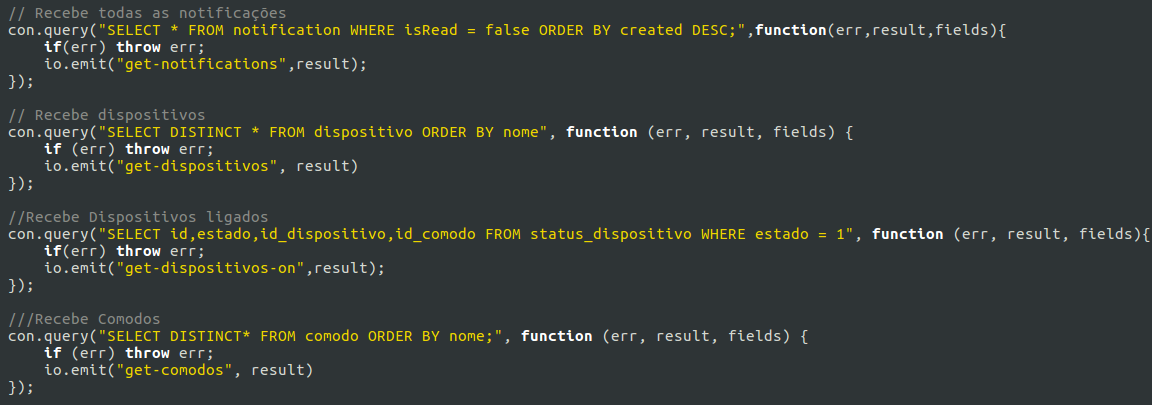
\includegraphics[width=1.0\textwidth, keepaspectratio=true]{api}
	\centering
	\caption[Chamada de API]{Chamada de API}
	\label{fig:api-ft}
\end{figure}
\FloatBarrier

\section[\textit{Hardware}]{\textit{Hardware}}\label{hard-sec}
\section[\textit{Resultados}]{\textit{Resultados}}\label{resultados-sec}
